\section{Solution implementation}
Here we discuss the implementation of our solution. As already anticipated,
the core of the system is a microservice architecture that communicates
through the REST API. Since every microservice is independent of each
other, the technologies that are used internally in the various modules
do not have to be the same ones. So, apart from keeping a standardized REST
interface among the components, we could develop the microservices with
different programming languages and frameworks. Here are described the
specific implementations of the single services.

\subsection{Microservices}


\subsection{User auth}

This module was built using Typescript that runs on a Node.js environment after
being compiled into Javascript. The corresponding database was built using MongoDB
that provides a NoSQL structure. The module uses the Express.js library to expose
its REST API and the Mongoose library to communicate with the database. The POST http
method was used to perform operations that edit entries in the database, such as
during the registration. The GET http method, instead, was used for operations that
do not modify content in the database, but only read information, such as the token
validation.\\

%\emph{http://user_auth_api:3000/[query]}\\

\begin{lstlisting}[language=bash,caption={User auth exposed API}]
    POST register
    JSON body data
        name: string
        surname: string
        email: string
        password: string
    JSON response
        token: string OR error: string
        
    POST login
    JSON body data
        email: string
        password: string OR token: string
    JSON response
        token: string OR error: string

    POST logout
    JSON body data
        email: string
        token: nullable string
    JSON response
        token: string OR error: string
        
    GET validate
    JSON body data
        email: string
        token: string
    JSON response
        token: string OR error: string
\end{lstlisting}


\subsection{Restaurant auth}

This module was implemented very similarly to the user auth one.

%\emph{http://restaurant_auth_api:3000/[query]}\\

\begin{lstlisting}[language=bash,caption={Restaurant auth exposed API}]
    POST register
    JSON body data
        name: string
        email: string
        password: string
    JSON response
        token: string OR error: string
        
    POST login
    JSON body data
        email: string
        password: string OR token: string
    JSON response
        token: string OR error: string

    POST logout
    JSON body data
        email: string
        token: nullable string
    JSON response
        token: string OR error: string

    GET validate
    JSON body data
        email: string
        token: string
    JSON response
        token: string OR error: string
\end{lstlisting}

\subsection{Restaurant data}
This module was build in python. Its corresponding database is build using MongoDB, which provides a NoSQL structure. Each restaurant is stored as a JSON object. The service uses the Flask library to expose the REST API and the pymongo library to communicate with the database. \\
The POST search method is used to search for a keyword among different restaurants. To overcome the MongoDB limitation of performing pattern matching for a nested object (the menu), each restaurant has a search\_string attribute which is a string containing all the items in the menu. \\
The GET search method is used to get a restaurant from its unique id. \\
Additionally there are two GET methods, namely pin and pingdb, which are used to ping the server and the database to perform a health check. These methods are not exposed. 


\begin{lstlisting}[language=bash,caption={Restaurant data exposed API}]
    POST search
    JSON body data
        query: string
    JSON response
        restaurants: list of json OR error: string
        
    GET search
    JSON body data
        id: string
    JSON response
        restaurant: json OR error: string
\end{lstlisting}


\subsection{Booking}
% Booking description here
This microservice module was completely written in python leveraging mainly the flask library to implement a REST API interface. Another technology that we used is MongoDB NoSQL database to store reservation records. As for the other services, database and applications logic are deployed in 2 different container. Apart from utilities methods such as ping the database or the microservices itself, the method that the service offers, following the design choices, are:

\begin{lstlisting}[language=bash,caption={Booking exposed API}]
    POST reserve
    JSON body data
        email: string
        authToken: string
        rest_email: string
        date: string
        service: string in {'lunch' or 'dinner'}
        time: string
        seats: int
        notes: string
        status: string in {'pending'[DEFAULT],'accepted','refused'}
    JSON response
    	body : "reservation pending"
        reservation_id: string
        OR error: string
        
    PATCH change_status
    JSON body data
        res_id: string
        status: string in {'pending','accepted','refused'}
        authToken: string
        email: string        
    JSON response
        res: "Status Updated" OR error: string
        
   POST my_reservations
   JSON body data
        email: string
        authToken: string
        user_type: int [0 -> user, 1 -> restaurant]
    JSON response
        list of reservation records OR error: string
\end{lstlisting}


\subsection{Web application}
For the purpose of the project, we also implemented a web application that serves
as a showcase to test the functionalities of our system. The backbone of our website
is composed of elements of HTML and CSS, tied up using \href{https://vuejs.org/}{Vue.js}
to add the responsive component. To enforce types, we opted to use TypeScript
in strict mode instead of the plain Javascript. We decided to use
\href{https://en.wikipedia.org/wiki/Ajax_(programming)}{AJAX} to send requests from the client to the servers. The interface is quite simple and implements the most important use cases that may be useful in the context of restaurant reservations, namely, we implemented the following use cases: user authentication, restaurant owner authentication, restaurant search using keywords, reserve a table, and handle an incoming user booking for a table. For a full description of how these functionalities are implemented please refer to their documentation in the microservices section. In particular, all requests that need to be authenticated are provided with an authentication token relative to the user session. Once the user is authenticated by our system, we store the authentication token that is provided by the user auth API in the local storage object. In this way, we are able to maintain the user session open even if the browser was closed. In such cases, we perform a technique known as silent sign-in using the above-cited token-based technique, enabling the user to proceed with their reservation transparently. For security reasons, we do not store user passwords on the client-side, neither encrypted ones, and the random generation of authentication tokens is performed on the server-side. Moreover, the website allows the non-authenticated user to view all available restaurants and see the details of a particular one, exception made for the booking request that can only be performed by a user that is currently logged into the system. A logged user can also see the list of their reservations, that have to be accepted by a registered restaurant owner. On the other side, we allow restaurateurs to see the collection of pending reservations that need to be accepted. Once the status of the reservation is changed on the restaurant side, the change is reflected in the user dashboard as well. It's worth noting that even though in this context the web application is only used to test the real system functionalities (implemented in the back-end), future work could be in the direction of improving the user experience on the website.
Two example pages are shown in Figure \ref{fig:explore_page} and Figure \ref{fig:booking_page}.

\vspace{0.5in}

\begin{figure}[H]
    \begin{center}
        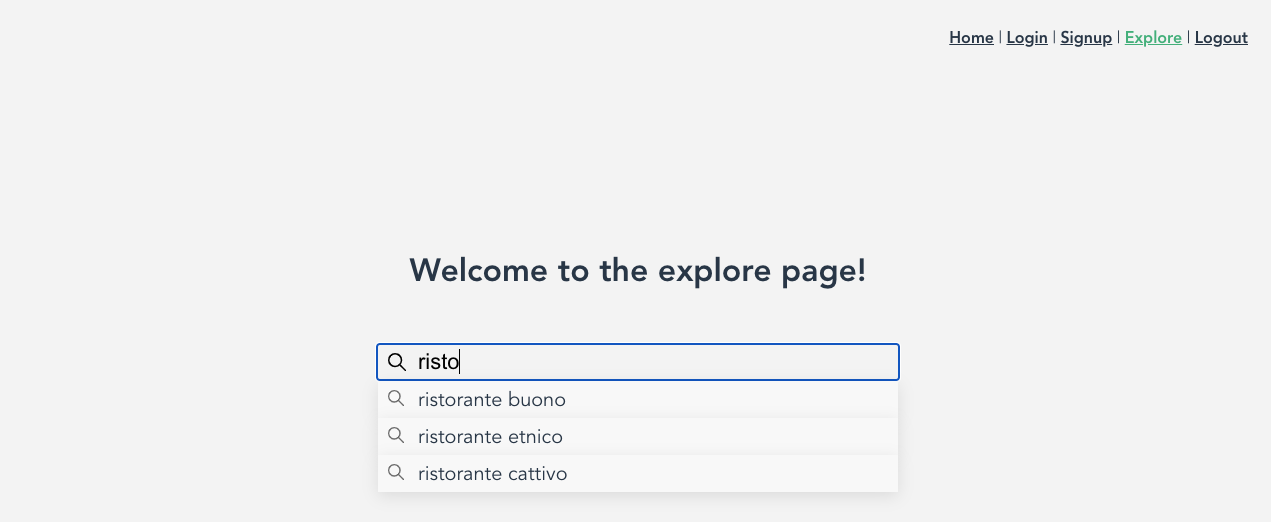
\includegraphics[width=8cm]{./images/explore_page.png}
    \end{center}
    \caption{Web app explore page.}
    \label{fig:explore_page}
\end{figure}

%\begin{figure}[H]
%    \begin{center}
%        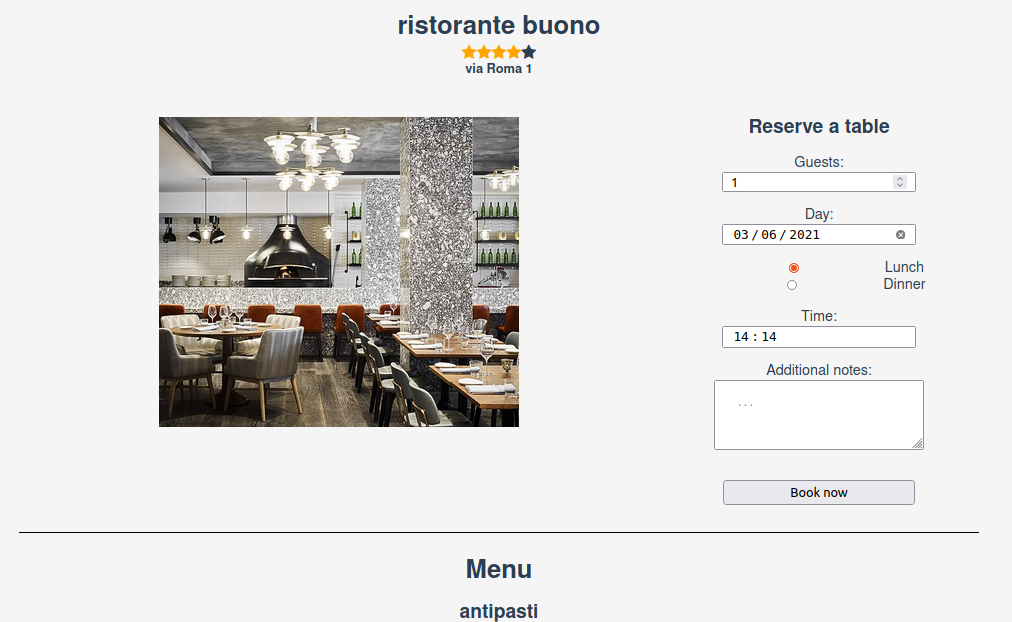
\includegraphics[width=8cm]{./images/reserve.png}
%    \end{center}
%    \caption{Web app booking page.}
%    \label{fig:booking_page}
%\end{figure}
%
%\begin{figure}[H]
%    \begin{center}
%        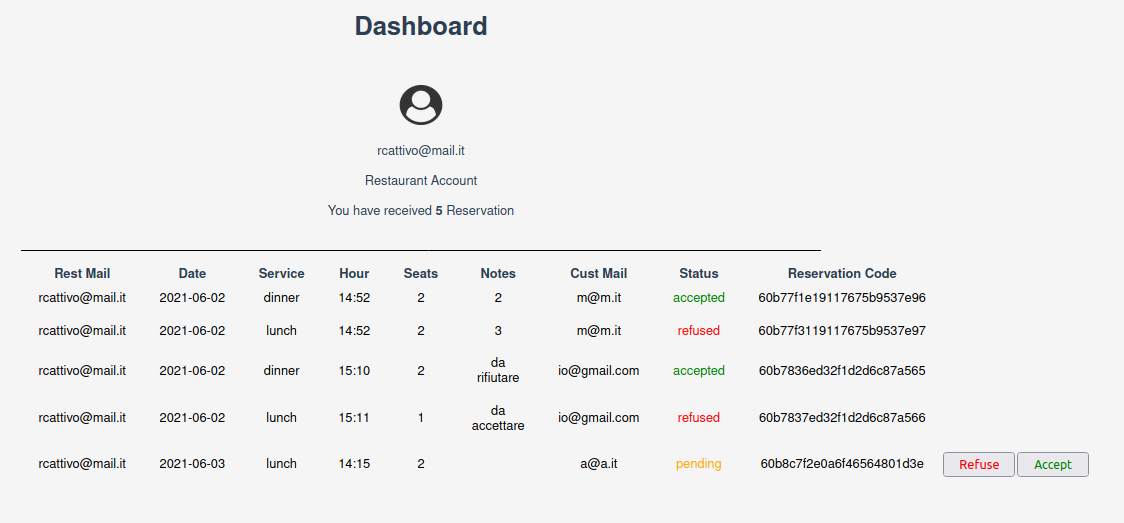
\includegraphics[width=8cm]{./images/dash.png}
%    \end{center}
%    \caption{Web app booking page.}
%    \label{fig:booking_page}
%\end{figure}

\textbf{Note: }\textit{ To try our webapp and see all the microservices at work, please clone our git repository, compile with make, and run docker-compose up --build. WebServer is running locally on port 8081. A demo video sample is available \href{https://www.youtube.com/watch?v=2iVW3yifJOw}{here}.} \clearpage

